 \section{Results and logs}
\label{sec:Results_and_Logs}

\subsection{Results}
When executing a COMPSs application we consider different type of results:
\begin{itemize}
 \item \textbf{Application Output:} Output generated by the application.
 \item \textbf{Application Files:}  Files used or generated by the application.
 \item \textbf{Tasks Output:} Output generated by the tasks invoked from the application.
\end{itemize}

Regarding the application output, COMPSs will preserve the application output but will add some pre and post output to indicate
the COMPSs Runtime state. Figure \ref{fig:compss_out} shows the standard output generated by the execution of the 
Simple Java application. The green box highlights the application \texttt{stdout} while the rest of the output is produced by COMPSs.  
\begin{figure}[!ht]
  \centering
    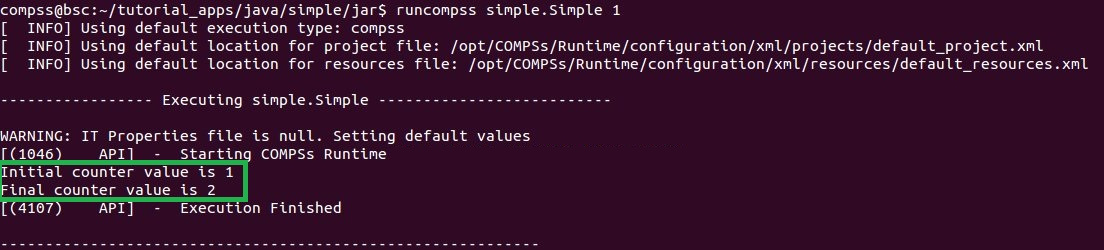
\includegraphics[width=0.95\textwidth]{./Sections/3_Results_and_Logs/Figures/simple_java_stdout.jpeg}
    \caption{Output generated by the execution of the \textit{Simple} Java application with COMPSs}
    \label{fig:compss_out}
\end{figure}

Regarding the application files, COMPSs \textbf{does not modify} any of them and thus, the
results obtained by executing the application with COMPSs are the same than the ones generated by the sequential execution
of the application.

Regarding the tasks output, COMPSs introduces some modifications due to the fact that tasks can be executed in remote
machines. After the execution, COMPSs stores the \textit{stdout} and the \textit{stderr} of each job (a task execution) inside the\\ \textbf{\texttt{/home/\$USER/.COMPSs/\$APPNAME/\$EXEC\_NUMBER/jobs/}} directory of the main application node.

Figures \ref{fig:hello_seq} and \ref{fig:hello_compss} show an example of the results obtained from the execution of the \textit{Hello} Java 
 application. While Figure \ref{fig:hello_seq} provides the output of the sequential execution of the application (without COMPSs), Figure \ref{fig:hello_compss}
provides the output of the equivalent COMPSs execution. Please note that the sequential execution produces the \texttt{"Hello World! (from a task)"} message
in the \texttt{stdout} while the COMPSs execution stores the message inside the \texttt{job1\_NEW.out} file.
\begin{figure}[!ht]
  \centering
    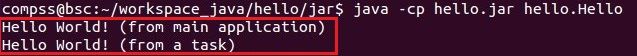
\includegraphics[width=0.7\textwidth]{./Sections/3_Results_and_Logs/Figures/hello_seq_stdout.jpeg}
    \caption{Sequential execution of the \textit{Hello} java application}
    \label{fig:hello_seq}
\end{figure}

\begin{figure}[!ht]
  \centering
    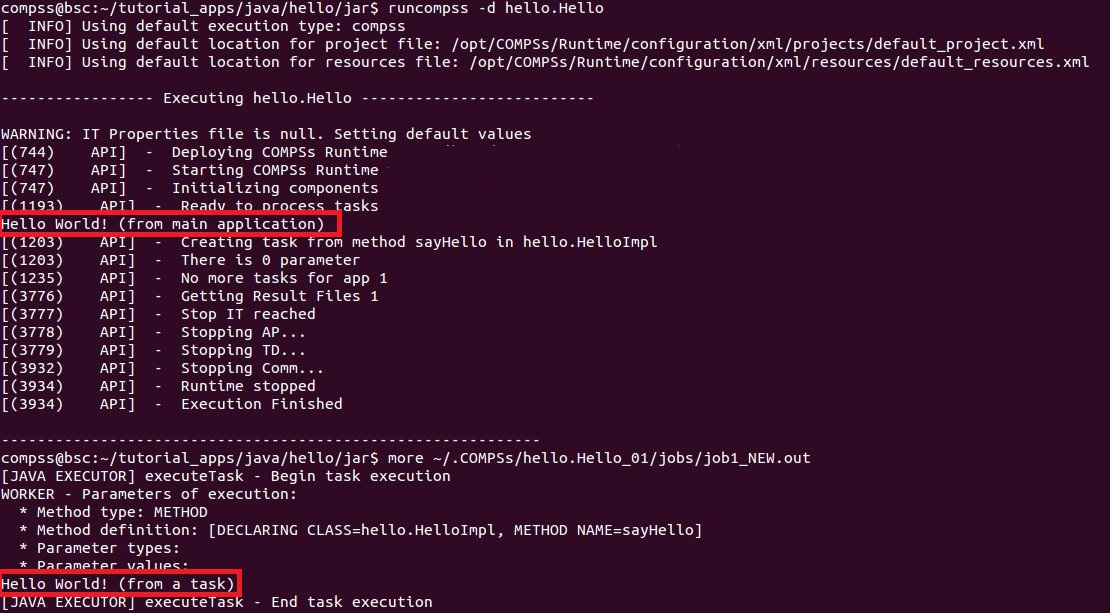
\includegraphics[width=\textwidth]{./Sections/3_Results_and_Logs/Figures/hello_compss_stdout_and_job.jpeg}
    \caption{COMPSs execution of the \textit{Hello} java application}
    \label{fig:hello_compss}
\end{figure}
\newpage

\subsection{Logs}
COMPSs includes three log levels for running applications but users can modify them or add more levels by editing the
logger files under the \verb|/opt/COMPSs/Runtime/configuration| \verb|/log/| folder. Any of these log levels can be selected by 
adding the \texttt{--log\_level=<debug | info | off>} flag to the \texttt{runcompss} command. The default value is \texttt{off}.

The logs generated by the \texttt{NUM\_EXEC} execution of the application APP by the user USER are stored under
\texttt{/home/\$USER/.COMPSs/\$APP/\$EXEC\_NUMBER/} folder (from this point on: \textbf{base log folder}). The \texttt{EXEC\_NUMBER} execution number is 
automatically used by COMPSs to prevent mixing the logs of data of different executions. 

When running COMPSs with \textbf{log level off} only the errors are reported. This means that the \textit{base log folder} will 
contain two empty files (\texttt{\textbf{runtime.log}} and \texttt{\textbf{resources.log}}) and one empty folder (\texttt{jobs}). If somehow the 
application has failed, the \texttt{runtime.log} and/or the \texttt{resources.log} will not be empty and a new file per 
failed job will appear inside the \texttt{jobs} folder to store the \texttt{stdout} and the \texttt{stderr}. 
Figure \ref{fig:simple_log_off} shows the logs generated by the execution of the Simple java application (without errors) 
in \textbf{off} mode. 
\begin{figure}[!ht]
  \centering
    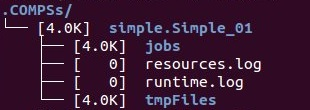
\includegraphics[width=0.4\textwidth]{./Sections/3_Results_and_Logs/Figures/simple_log_off.jpeg}
    \caption{Structure of the logs folder for the Simple java application in \textbf{off} mode}
    \label{fig:simple_log_off}
\end{figure}

When running COMPSs with \textbf{log level info} the \textit{base log folder} will contain two files (\texttt{\textbf{runtime.log}} and 
\texttt{\textbf{resources.log}}) and one folder (\texttt{jobs}). The \texttt{\textbf{runtime.log}} file contains the execution information retrieved 
from the master resource, including the file transfers and the job submission details. The \texttt{\textbf{resources.log}} file contains 
information about the available resources such as the number of processors of each resource (slots), the information about running or 
pending tasks in the resource queue and the created and destroyed resources. The jobs folder will be empty unless there has been a
failed job. In this case it will store, for each failed job, one file for the \texttt{stdout} and another for the \texttt{stderr}.
As an example, Figure \ref{fig:simple_log_info} shows the logs generated by the same execution than the previous case 
but with \textbf{info} mode. 
\begin{figure}[!ht]
  \centering
    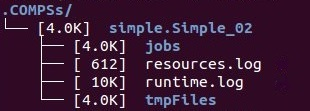
\includegraphics[width=0.4\textwidth]{./Sections/3_Results_and_Logs/Figures/simple_log_info.jpeg}
    \caption{Structure of the logs folder for the Simple java application in \textbf{info} mode}
    \label{fig:simple_log_info}
\end{figure}

The \texttt{runtime.log} and \texttt{resources.log} are quite large files, thus they should be only checked by advanced users. For an
easier interpretation of these files the COMPSs Framework includes a monitor tool. For further information about the COMPSs Monitor
please check Section \ref{subsec:monitor}.

Figures \ref{fig:simple_runtimelog} and \ref{fig:simple_resourceslog} provide the content of these two files generated
by the execution of the \textit{Simple} java application. 
\begin{figure}[!ht]
  \centering
    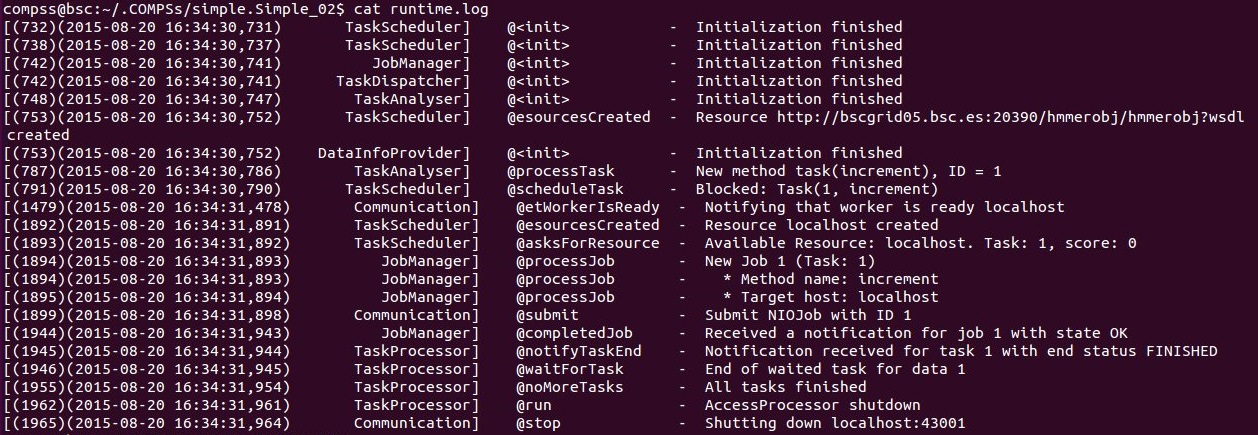
\includegraphics[width=0.95\textwidth]{./Sections/3_Results_and_Logs/Figures/simple_runtimelog.jpeg}
    \caption{runtime.log generated by the execution of the \textit{Simple} java application}
    \label{fig:simple_runtimelog}
\end{figure}

\begin{figure}[!ht]
  \centering
    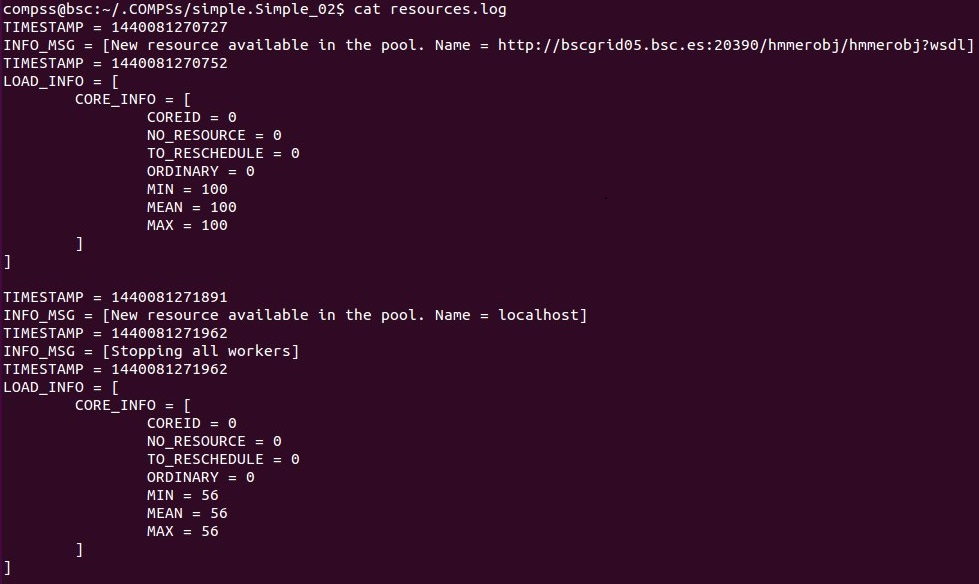
\includegraphics[width=0.95\textwidth]{./Sections/3_Results_and_Logs/Figures/simple_resourceslog.jpeg}
    \caption{resources.log generated by the execution of the \textit{Simple} java application}
    \label{fig:simple_resourceslog}
\end{figure}

Running COMPSs with \textbf{log level debug} generates the same files as the info log level but with more detailed information.
Additionally, the \texttt{jobs} folder contains two files per \textbf{submitted} job; one for the \texttt{stdout} and another for
the \texttt{stderr}. In the other hand, the COMPSs Runtime state is printed out on the \texttt{stdout}. Figure 
\ref{fig:simple_log_debug} shows the logs generated by the same execution than the previous cases 
but with \textbf{debug} mode. 

The runtime.log and the resources.log files generated in this mode can be \textbf{extremely large}. Consequently, the users should
take care of their quota and manually erase these files if needed. \newline

\begin{figure}[!ht]
  \centering
    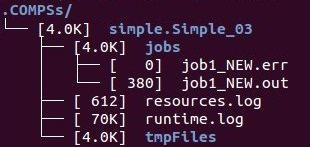
\includegraphics[width=0.4\textwidth]{./Sections/3_Results_and_Logs/Figures/simple_log_debug.jpeg}
    \caption{Structure of the logs folder for the Simple java application in \textbf{debug} mode}
    \label{fig:simple_log_debug}
\end{figure}

When running Python applications a \texttt{pycompss.log} file is written inside the \textit{base log folder} containing debug
information about the specific calls to PyCOMPSs. 

Furthermore, when running \texttt{runcompss} with additional flags (such as monitoring or tracing) additional folders will appear inside the 
\textit{base log folder}. The meaning of the files inside these folders is explained in Section \ref{sec:Tools}. 
